% !TeX encoding = UTF-8
\documentclass[journal,comsoc]{IEEEtran}
% \documentclass[journal,comsoc]{../sty/IEEEtran}
\usepackage{graphicx,times,amsmath,booktabs,algorithm,algorithmic,amsmath}
\usepackage{multicol}
\usepackage{amsmath,amssymb}
\usepackage{subfigure}
\usepackage{hyperref}	
\usepackage{url}
\usepackage[T1]{fontenc}% optional T1 font encoding
\usepackage[cmintegrals]{newtxmath}

% Article
\begin{document}
	
	\title{Neuron Analogy Network}
	%		\title{Bio-Inspired Heterogeneous Wireless Networks Design: A Neuron Analogy Perspective }
	
	\author{Quan~Yu,~\IEEEmembership{Fellow,~CAE}}	
	\markboth{Journal of Communication,~Vol.~14, No.~8, December~2018}%
	{Shell \MakeLowercase{\textit{et al.}}: Bare Demo of IEEEtran.cls for IEEE Communications Society Journals}
	\maketitle
	
	\begin{abstract}
		Recently, heterogeneous wireless network(HWN) is attracting lots of research attention in multiple fields with the development of 4G, internet of vehicles, internet of things, etc. 
		However, with the mobility and increasing number of nodes, the performance of HWN would decrease exponentially due to the time-varying of network topology and uncertainty of service requirement. 
		In this paper, we primarily introduce the information transmission mechanism of neural netwroks, 
		and compare the mechanisim with that of HWN in detail, 
		including the node model, network structure, and transmission protocol. 
		Furthermore, we propose the neuron analogy heterogenous wirelss network(NANET) initially and provide its overall design of node and network architecture simultaneously as well.
		In addition, we depict the macroscopic goals of NANET  and related feasible technologies that might be applied in the future.
	\end{abstract}
	
	\begin{IEEEkeywords}
		Neuron Analogy Heterogenous Wireless Network, NANET, 
		%		Heterogenous Wireless Networks,
		Information Transmission Mechanism
	\end{IEEEkeywords}
	
	\IEEEpeerreviewmaketitle
	
	\section{Introduction}
	\label{section: introduction}
	\IEEEPARstart{H}{eterogeneous} wireless network(HWN) is a distributed, self-organizing, and heterogeneous network without unique center.
		Recently, it have been envisioned to play a crucial role in the future networks, 
		such as vehicle2vehicle(v2v)/vehicle2instrument(v2i), sensor networks, 5G/B5G, military communication network, and so forth.
		
		Neuron Analogy Networks(NANETs) is a heterogeneous wireless network, which consists of a collection of wireless mobile nodes (or routers) dynamically forming a temporary network without the use of any existing network infrastructure or centralized administration.
		
		NANETs don't maintain a fixed infrastructure, but it can provide communication between terminals without using or making use of existing network infrastructures.
		The routers are free to move randomly, and yet the network can organize themselves freely. 
		Thus, the wireless network topology may change rapidly and unpredictably. 
		Such a network may operate in a standalone fashion, or may be connected to the Internet. 
		Some form of routing protocol is in general necessary in such an environment, 
		since two hosts that may wish to exchange packets might not be able to communicate directly.
		
		At present, a lot of works have conducted research on information networks and accomplished certain achievements.
		Jinyang Li et al. studied the capacity of AdHoc networks.
		Work by Matthias Grossglauser et al. believes that mobility increases the capacity of Ad Hoc networks.
		Rudolf Ahlswede et al. proposed the theory of network coding to increase the capacity of a multicast network by coding the received information through relay nodes.
		*** Researched 3C fusion theory, transmission, calculation, storage in one, and achieved certain results, has been widely used.
		EM Royer summarizes the routing protocols in Ad hoc networks.
		However, these studies were mainly applied at the engineering level and didn;t reach the theoretical height of Shannon's "information theory." \par
		
		Therefore, there does exit effects on the information network just as the influence of network structure, node structure, encoding method, and routing protocol.
		The combination of those multiple factors has cause great trouble for us to systematically resolve the problems HWN networks confronting.
		
		
		
		In this paper, we will systematically propose a neuron analogy heterogeneous networks architecture, analogous to human neuronal networks, to settle or alleviate current challenges the HWN facing.
		
		The remainder of the paper is organized as follows. 
		In Section \ref{section: research_challenges}, we depict current challenges in HWN.
		In Section \ref{section: information_transmit}, we introduce the information transmit model of the neural networks 
		and make analogies between neural networks and HWN in Section \ref{section: analogy}.
		Then, in Section \ref{section: framework}, we propose the general design and goals of NANET.
		Finally, we conclude the paper in Section \ref{section: Conclusion}.
		
	\section{Challenges of Heterogeneous Wirelss Networks}
	\label{section: research_challenges}
		In general, HWNs are confront with many challenges, 
		which mainly come from the characteristics of network nodes, the network architecture, 
		the environmental conditions of the channels, and the service demands of users.
	
	\subsection{Mobility of Network Node}
		As for the nodes of HWN,  they moves frequently with a wide scale of moving speed but without regular movement rules, 
		which leads great difficulty to model the behaviors of network nodes.
		The core problem of HWN is the mobility, which always results in tremendous overhead of routing protocol. 
		However, what's terrible is that when the network is in a bad status, mobility would make it even worse. 
		Because the faster the network framework changes, the larger the signaling overhead of mastering the state of the network.
		And meanwhile, uncertain movements of nodes implies fast and unpredictable changes in the network topology, throughput, load, etc. 
		If employing traditional network architecture and routing protocol, the time-varying network topology will cause tremendous routing overheads, 
		making it difficult to content users' demands for network traffic, service, and stability included.
	
	\subsection{Network Architecture}
	
		\subsubsection{Heterogeneity of Network Topology}
			One of the distinguishing features of the HWNs is the heterogeneity of the network structure.
			We expect that the network will have a variety of capabilities and complex network framework to deal with problems caused by nodes' movements  and meet the quality of service(QoS).
			Thus, conflicts brought by heterogeneity and the complexity appear at this moment.
			The properties of heterogeneity and hierarchy will greatly increase the complexity of the network, 
			which will limit our ability to perceive and control the network.
			Along with the network's growing more and more complex and heterogeneous, it's becoming more and more difficult to master the network.
			Therefore, the heterogeneity and complexity of the network topology will bring great challenges to network managers.
			However, heterogeneity is not only a challenge but also an opportunity.
			It is hard for a homogeneous network to meet the complicated needs of the network's services. 
			To some extent, a network would become heterogeneous inevitably as 4G, vehicle networks, and sensor networks have done.
			Therefore, 	we should also do research on a universal framework to deal with the challenges that heterogeneity bring tp us while emploiting the heterogeneity of the network to bring convenience to us.
			In essence, it is an engineering balance between the adaptability and the complexity brought by the heterogeneity.		
			
			\subsubsection{Time-variability and Uncertainty of Network Topology}
				HWN is a time-varying and uncertain network.
				With the movement of network node, the network topology is changing over time and correlative node speed.
				Time-variability determine that management of the HWN is much more complicated than that of wired network,
				because the dynamics of the network topology requires dynamic self-organizing and self-configures of network management system. 
				In the meantime, the type of service, and the traffic flow are uncertain, 
				which will engender an exponential decline of the network  performance.
				Considering the limitations of the mobile node itself, such as limited energy, transmission link status, 
				tiny bandwidth and restricted storage capacity, etc., 
				we should take into account the load brought by the management protocol to the entire network. 
				Besides, we must consider the applicability of network management to different environments.
		
		\subsection{Communication Channel}
			\subsubsection{Limited Bandwidth of Transmission Link}
				As for HWN, channel is always restricted due to the limited bandwidth of communication terminal.
				The physical characteristics of the wireless channel itself determine that the bandwidth of the mobile ad hoc network 
				is much lower than that of the wired channel. 
				Thus, the wireless channels are competitive and shared as well, which will result in competition for communication resources, 
				attenuation of wireless signals, noise interference, and interference due to channel characteristics.
				And then, all these conditions lead to the fact that the actual bandwidth available to the mobile terminal is far less than the theoretical bandwidth.
				It's tough for the bandwidth of transmission link to sustain to increase since the spectrum resources used for wireless transmission are limited(i.e., the capacity of the network is limited).
				Hence, it's  for HWN networks to fulfill the exponential growth of users' demands for network traffic.
			
			\subsubsection{Strong Wireless Channel Inference}
				The wireless channel is relatively uncertain in a sense.
				With more and more devices and terminals joinning in the wireless networks, it's becoming stronger and stronger for the mutual interference among devices simultaneously.
				In order to meet peformance and service requirements in 5G, operators are constructing a series of ultra-dense networks, 
				which greatly increases the interference between networks, for example, the neighborhood interference.
				At the same time, the continuous development of networks, such as sensor networks, smart power grids, vehicle networks, etc., 
				the significant interference within the HWN . 
				All these interferences will have an adverse effect on the channel environment and performance indicators( BER and SNR). 
				which subsequently makes stupendous trouble on guarantee of network performance and quality of service.
		
		\subsection{Diversity of Network Service}
			Demands of Service in HWN are diverse. 
			The network is always required to be capable of providing a wide variety of services, for instance, voice, data transmission, streaming media, and etc.
			So it's a hard work for a network with a variety of services loaded on, to ensure the quality of various services.
			And there is a wide gap between the demands of different services, which further increase the complexity of the network.
			That is, the diversity of services is always of great uncertainty in HWN.
			Consequently, the guarantee of network's QoS remains a awkward and urgent problem.
			
			The time-diversity and uncertainty of channel, node status, topology, service, and traffic, 
			result in the performance of HWN network to decrease exponentially with the number and mobility of nodes.
			Thus, there are many issues for researchers to work on, 
			which mainly concentrates on the design of network node, network architecture, and transmission protocol.
	
	\section{Overview of Biological Neural Networks}
	\label{section: information_transmit}
		Brain is the command center for the human nervous system\cite{hart1983human}.
		As \cite{rsheng} noted, the nervous network achieves the basic function of signal transduction and information transmission with specialized characteristics.
		Although everyone's nerons are the similar, there will be many amazing creativities when cells connecting and forming a trillion-dollar link.
		In this section, we'll discuss the basic characteristics of neural network in three issues: the neuron node, the  information transmission between neuron nodes, and the neural network.
		
		\subsection{General Characteristics of Neurons}
		
			\subsubsection{Structure Characteristics of Neurons}
				In order to simplyfy the recognition for neuron, we merely elaborate with a typical structure of neuron as shown in Fig. \ref{fig: neuron_cell}.
				\begin{figure*}[htbp]
					\centering
					\subfigure[Canonical Neuron model.]{
						\begin{minipage}[c]{0.46\linewidth}
							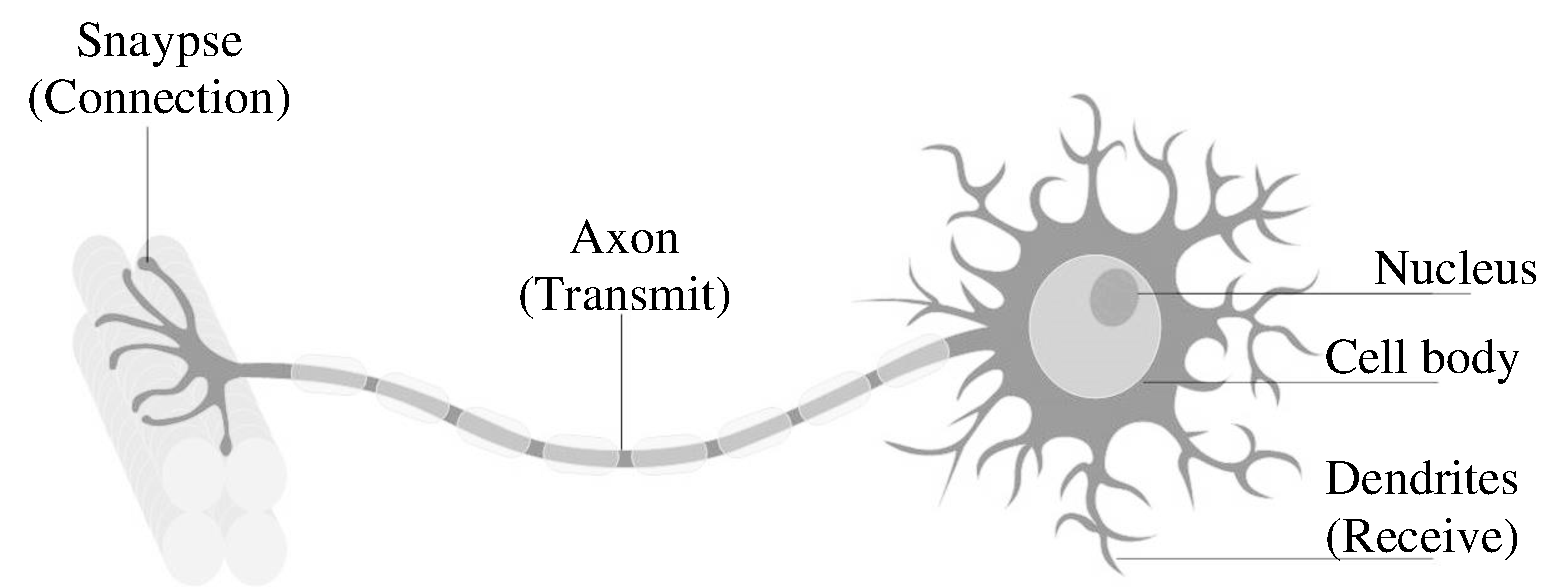
\includegraphics[width=3.5in]{figures/neuron.pdf}
							\label{fig: neuron_cell}
					\end{minipage}}
					\subfigure[The heterogeneity of neurites.]{
						\begin{minipage}[c]{0.46\linewidth}
							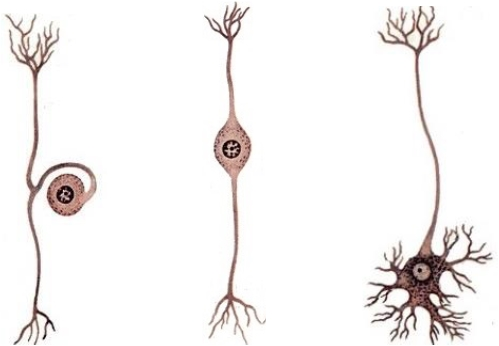
\includegraphics[width=3.3in]{figures/node_het}
							\label{fig: node_het}
					\end{minipage}}
					\caption{Heterogeneity and Structure Features of Neurons.}
				\end{figure*}
				As shown in Fig. \ref{fig: node_het}, there are mainly three types of neurons based on shape and number of neurites: the unipolar, bipolar and multipolar neurons\cite{bear2007neuroscience}. 
				In general, neuron contains at least two distinguishable parts: a central region including the cell body, and multiple neurites radiating away from the cell body. 
				Inside the neuron cell body, the cytoskeleton, consisting of microtubules, microfilaments, and neurofilaments, shapes the neuron cell and regulates itself dynamically. 
				What's called the synapse is the junction between the axon of the previous neuron and the dendrites of the next neuron.
				With regard to the neurite, it consists of two types: axons and dendrites (fig. \ref{fig: neuron_cell}), which are separated in a neuron cell obviously.
				The cell body usually comes into being merely a single axon which can extend over great distances from the cell body (a meter even longer).
				However, dendrites typically branch profusely, getting thinner with each branching, and usually not exceeding 2mm from the cell body.
		
			\subsubsection{Overview of Neurites}
				Information in neurite is first transmitted on an axon, and then delivered separately with its bifurcation at axon terminals. 
				Axon typically extends some distance from the cell body and carries signals to other neurons.
				It always forwards electrical impulses along the axon proper and passes them to other innervated neurons through synaptic contact. 
				Therefore the signal in neuron transmits from one axon to multiple dendrites in the form of an internal broadcast, which manifests a non-selective feature.
				Dendrites usually branch out in tree-like fashion, and are the main apparatus for receiving incoming signals from other nerve cells. 
				Each of dendrites has its own direction of reception and is responsible for the information acception in this direction, which means that the reception is directional. 
				In addition, we can also find that the information is merged in each small branch point and then transmitted to the cell body.			
			
			\subsubsection{Information Processing in Neurons}
				The generation of action potential is based on the parallelled information fusion and processing in the cell body through weighing the consequences of input local signals and then deciding whether to generate an action potential. 
				When the sum of depolarizations produced by the local signals surpasses a certain voltage threshold, the sodium ion channels in the cell membrane are open and generate an action potential at the trigger zone. 
				In biological neuron, there exits a kind of excitable membrane that is able to keep action potential with fixed strength and duration once it has been generated.
				Eventually, information is encoded with the frequency of action potentials as well as number and combination of action potentials from different neurons\cite{bear2007neuroscience}. 
				
		\subsection{Overall Characteristics of Neural Networks}
			The development of brain science has enabled us to study the structure of the human brain and corresponding mechanism of information transmission.
			
			\subsubsection{Information Transmission between Neurons}
				A synapse is the specialized junction where one part of a neuron joint and communicates with another neuron or cell type (such as a muscle or glandular cell). 
				In the nervous system, information transmission are generally classified into two categories: electric synapse transmission and chemical synaptic transmission.
				Fig. \ref{fig: synaptic_cop} presents the comparison of chemical synaptic trianmission and electric synapse transmission.
				\begin{figure}[htbp]
					\centering
					\subfigure[electric synapse transmission.]{
						\begin{minipage}[t]{0.48\linewidth}
							\centering
							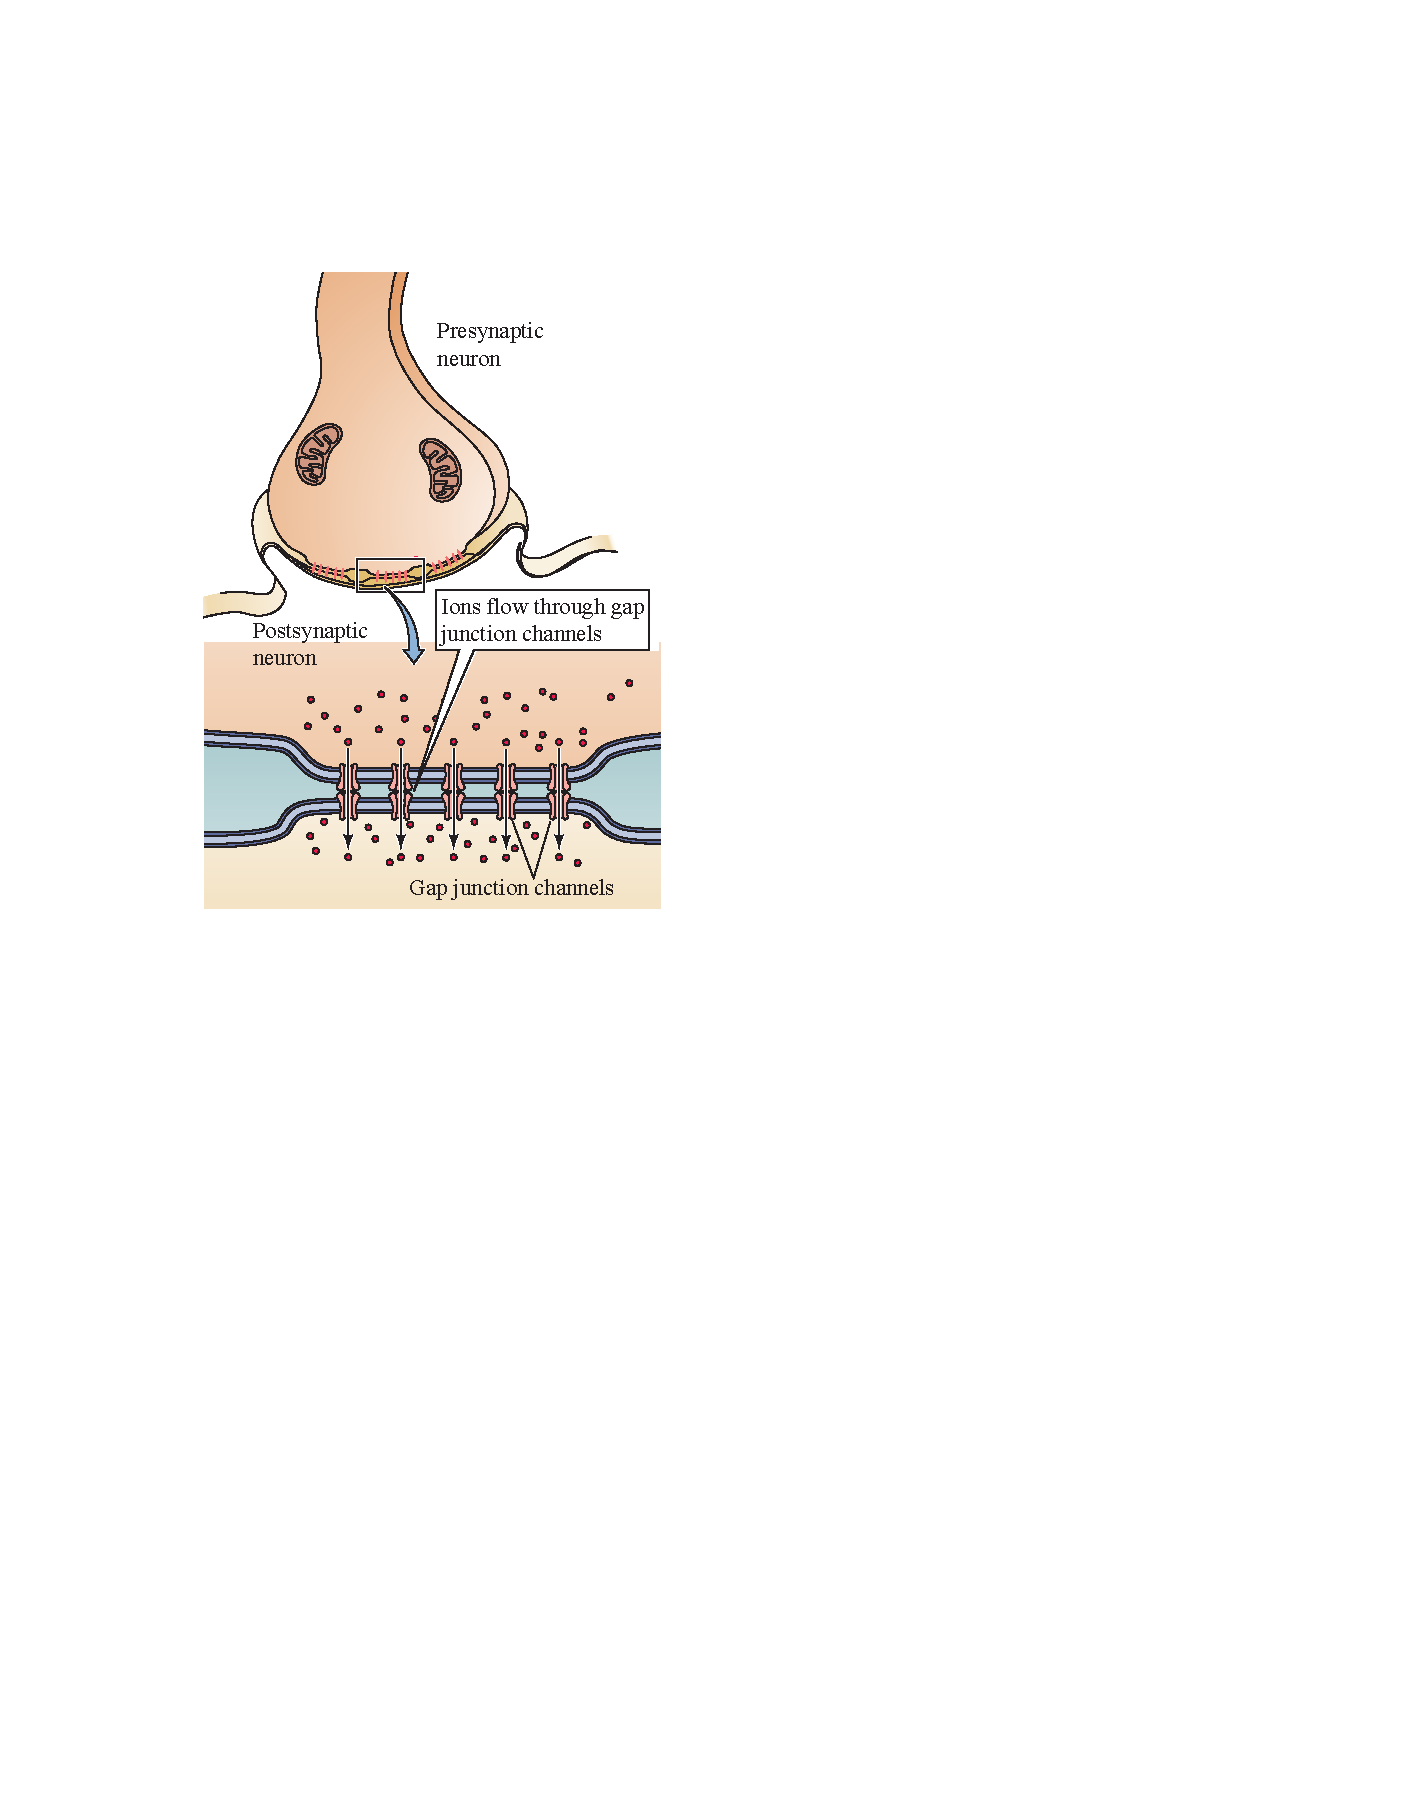
\includegraphics[width=\linewidth]{figures/electronic_trans.pdf}
							\label{fig: electronic_trans}
					\end{minipage}}
					\subfigure[Chemical synaptic transmission.]{
						\begin{minipage}[t]{0.48\linewidth}
							\centering
							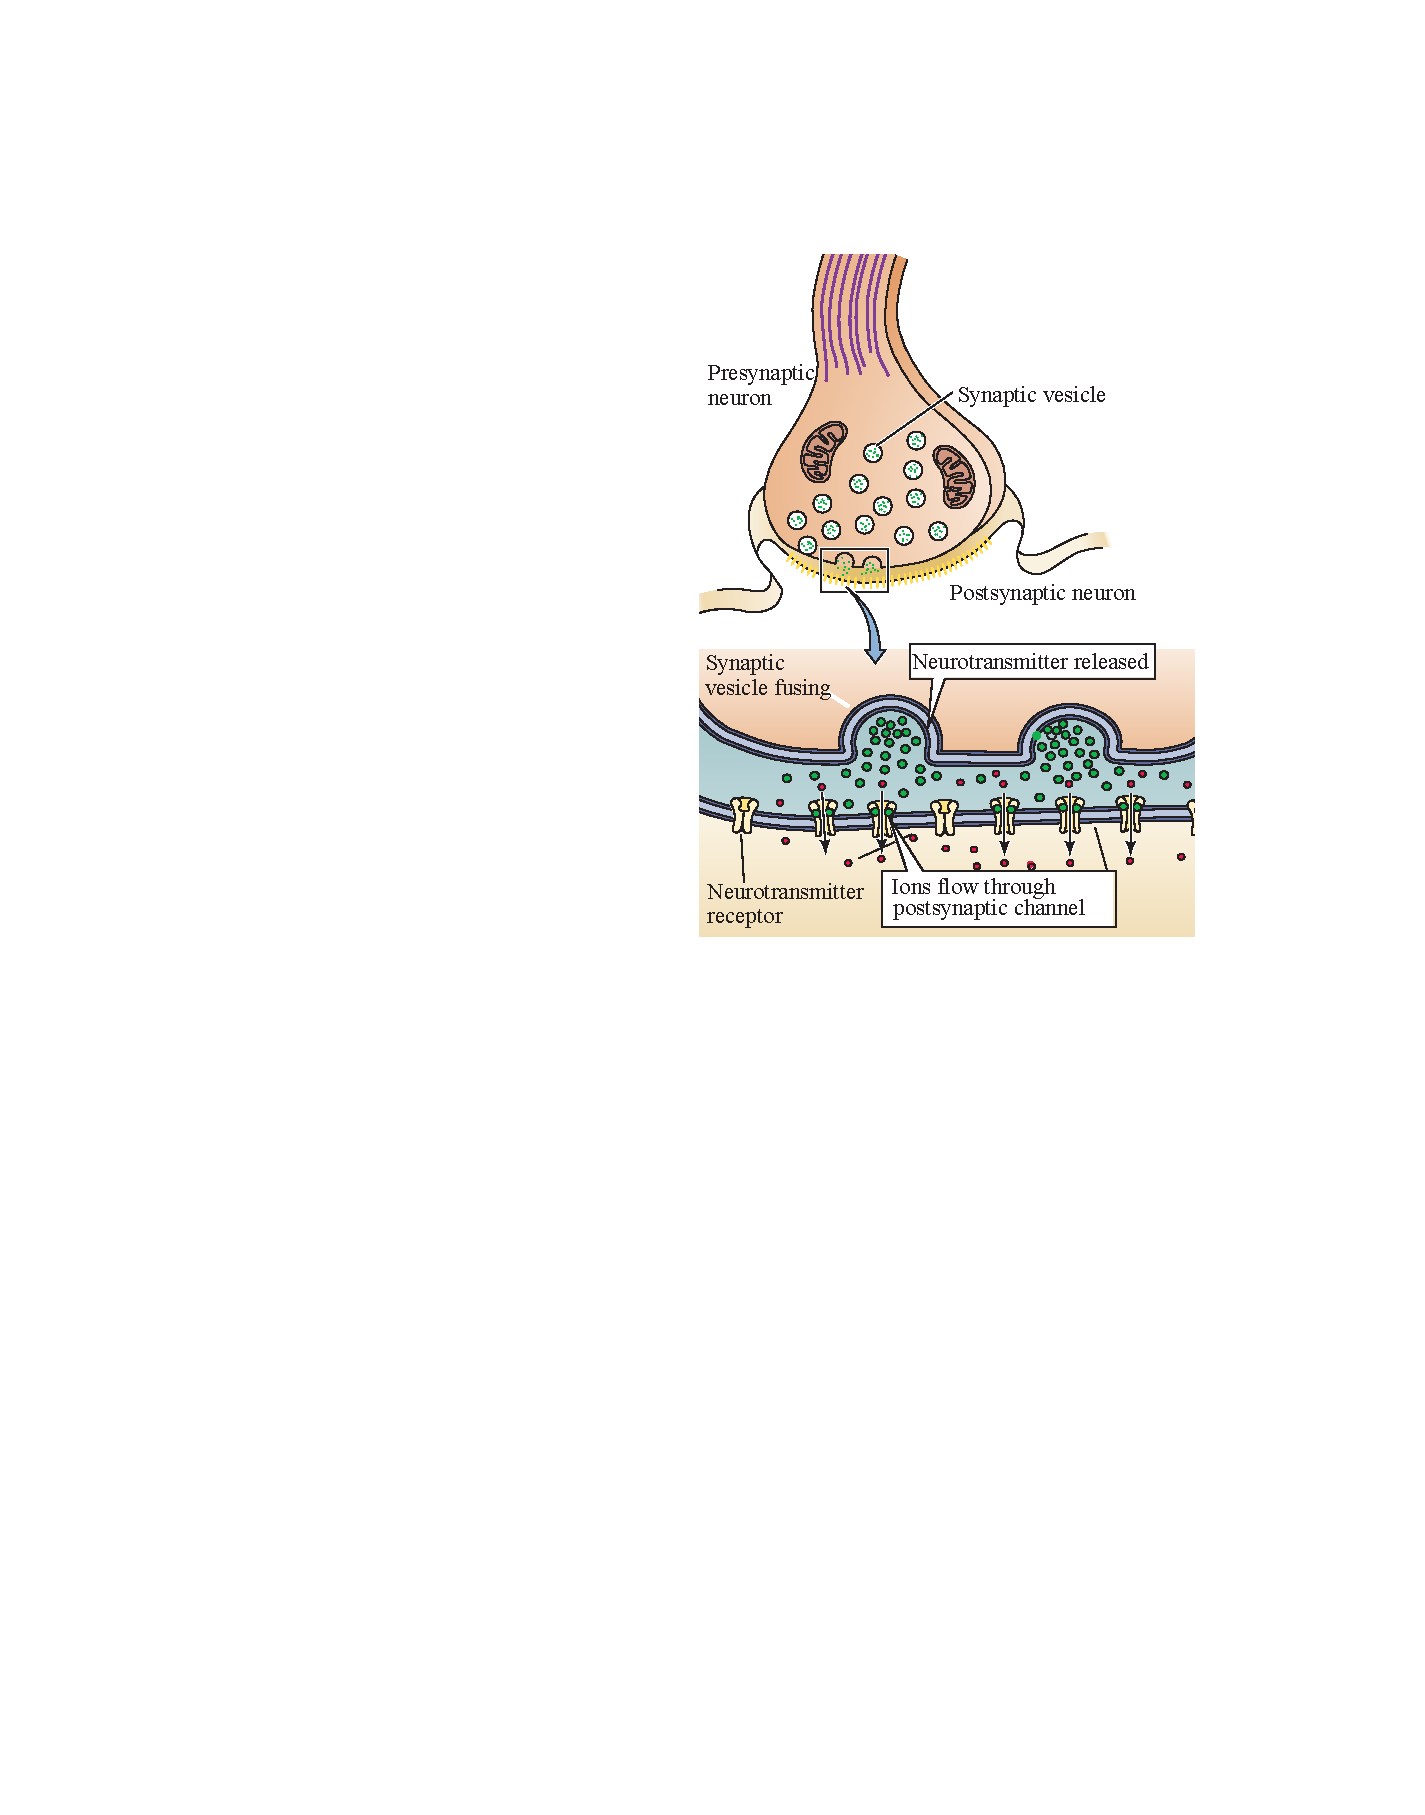
\includegraphics[width=\linewidth]{figures/chemical_trans.pdf}	
							\label{fig: chemical_trans}
					\end{minipage}}
					\caption{The comparision of chemical synaptic trianmission and electric synapse transmission.}
					\label{fig: synaptic_cop}
				\end{figure}
			
				As shown in Fig. \ref{fig: chemical_trans}, the presynaptic is usually composed by axon terminal, and presynaptic and postsynaptic membranes are separated by a synaptic cleft.
				Most neurons receive multiple synaptic inputs that activate different combinations of ion channels and receptor proteins. 
				The postsynaptic neuron integrates all these complex ionic and chemical signals to produce the action potentials\cite{beanewman2003structure007neuroscience}. 
				Synaptic integration constitutes the neural computation for transformation of many synaptic inputs to a single neuronal output, by which multiple synaptic potentials combine within one postsynaptic neuron.
				The neuron is firing action potentials at a high rate, and because many synapses were activated at the same time, activations summed to bring the spike-initiation zone of the postsynaptic neuron to threshold, and this cell then generated action potentials. 
				
				As shown in Fig. \ref{fig: electronic_trans}, a gap junction interconnecting the dendrites of two neurons constitutes an electrical synapse.
				An action potential generated in one neuron causes a small amount of ionic current to flow through gap junction channels into a second neuron, 
				inducing an electrical postsynaptic potential.	
				Most gap junctions allow ionic current to pass equally well in both directions.
				Therefore, electrical synapse transmission is bidirectional which is different from the vast majority of chemical synapses.
				Transmission at electrical synapses is very fast and, and it can approach the speed of light in a idle condition. 
				
				Generally, neuronal cells receive thousands of synaptic inputs that activate different combinations of receptor proteins and their corresponding ion-gated channels on the cell surface.
				It namely means that neuronal information transmission is related to combination of activated channels and receptor proteins, which is similar to the network coding in our information network. 
				Through the information transmission between multiple network nodes, it is allowed to encode and fuse the information from different links. 
				Thus, the combination of all link information constitutes the complete information.		
				
			\subsubsection{A Scale-free Network Structure Subjected to Power-law Distribution}
			
				In terms of network scale, the neural network obeys the so-called power law distribution (scale-free) that has a certain structural universality\cite{bibid}.
				The range of neuronal network signal transmission is large-scale changes, and the length of axons ranges from several micrometers to more than one meter which is a difference of nearly a million times.
				Meanwhile, the neural networks is with short average path length, big clustering coefficient, and more clustered feature compared to random networks, which represents the small-world characterisctic in some sense\cite{eguiluz2005scale}
				As \cite{papo2014complex} noted, the brain neuron network shows small-world property at global level, non-random topological property at mesoscopic level, and centrality property at nodal level. 
			
			\subsubsection{Hierarchical and Heterogeneous Network Architecture}			
				On the one hand, the biological neural network is a hierachical network.
				For example, the cell bodies of cortical neurons are always arranged in layers, or sheets, that usually lie parallel to the surface of the brain\cite{bear2007neuroscience}.
				In addition, neurons in the cerebral cortex are organized in layers, including molecular layer, external granule cell layer, external pyramidal cell layer, internal granule cell layer, internal pyramidal cell layer and multiform layer. 
				On the other hand, the biological neural network is a heterogeneous network consisting of node heterogeneity and topology heterogeneity.
				From the perspective of node,  the heterogeneity is reflected on the structure and function.
				For instance, there are primarily three kind of node model as shown in Fig.\ref{fig: node_het}.
				And, there are three types of neurons according to function of synapses connection in motor nervous system, which are the primary sensory neurons, motor neurons and interneurons.
				From the perspective of topology, different functions and structure of nervous system reveals the heterogeneity.
				Conventionly, the human nervous system is anatomically divided into central and peripheral components, 
				and the brain functions are realized through interactions of neuron cells from heterogeneous topology (circuit or loop) with specific purposes\cite{kandel2000principles}.
				Consequently, we can conclude that biological neural network is a hierachical and heterogeneous network.
	
	\section{The Analogy between HWN Networks and Neural Networks}
	\label{section: analogy}
		The traditional communication mainly focuses on point-to-point communication.
		However, in the information network, especially the Internet, point-to-point communication has been negligible. 
		Thus, we are more concerned with proliferation and sharing of information.
		In this section, we will compare the HWN network with the neural network from three aspects: the node model, the transmission protocol between nodes, and the network architecture as well.
		
		\subsection{Analogy of Node Model}
		\label{subsec: analogy_of_node_model}
			The neuron is mainly consisted of cell body and neurites, in which the neurites is in charge of information transmission and reception while the cell body is used to information processing and storage.
			Therefore, the information of neuronal cells is a trinity of transmission, coomputation, and storage.
			Moreover, the computation and storage are always integrated in a sense, conforming to the relevant theory of computer.
			As there are three chief shapes of neurons, each of which equips different function, we can strengthen a certain ability, such as transmission or computation, to reinforce considerding function of the neuron.
			In neural system, it employs the synapse for information interaction among different neurons, which resembles the combination of antenna and baseband processing unit in communication system.
			And the dendrites and axons are seperated, revealing the separation of transmission and reception in neuron cell. 
			The information is transmitted omnidirectionally by axon while it's received directionally by dendrites at the synapse.
			In dendrites, the information is gradually integrated hierachically, which means that the information is also processed while being transmitted,  and is then fused integrally at the inner of the neuron.
			Therefore, the information reception and fusion is parallelled processed within neuron cell, proving the parallel characteristic of information reception, fusion and processing.
			Meanwhile, the action potential remainds stationary when it's transmited after accomplishing the threshold with the accumulation of electric stimulus.
			Also, the information is coded by the firing rate and time, which is similar to the frequency modulation in wireless communication.

		\subsection{Analogy of Network Architecture}
		
			The human brain contains nearly 100 billion neuron cells, each of which has different shapes and functions.
			However, when these cells are connected in different ways, trillions of links are established.
			All of the neuron and links can be well coordinated to constitute the human's various nervous systems, and operate methodically.
			Hence, the stable mechanism of information transmission in such a large and complex system is of great reference value for our communication network.
			Comparing with biological neural network, the naturally forming HWN is a scale-free network subjected to power-law distribution, too.
			And, the majority of nodes and links possess a short average path length and can cluster in a relatively small locality subjected to small-world property.
			From the perspective of network framework, neural netwokr is a distributed and peer-to-peer network without a strict control center but with a stable backbone netowrk relatively.
			Simultaneously, both the neural network and HWN are hierachical and heterogeneous.
			At every second, there are thousands of new connections established and thousands of connections broken while more connections are modified at strength, 
			which appears that the neural network topology is rapidly changing and highly plastic.
			
		\subsection{Analogy of Transmission Protocol}
			    	
			In the information transmission of neurons, the traffic channel is separated from the control channel.
			The Service channel could be analogized to chemical synaptic transmission, while the control channel is analogous to the transmission of electric synapses transmission. 
			Information transfer in neuronal networks is generally dominated by chemical synaptic transmission, 
			whereas the electric synapses transmission  is often used as a synchronization mechanism for coordinating multiple sets of neuronal activities, which is similar to signaling protocols in communication networks.
			Since the electrical synapse applys the electron to transfer information, its' speed is extraodinarily fast than that of chemical synapse that employs the neurotransmitter with a delay of about one millisecond.
			The chemical synapse is collaborative for its abilities of fusing and processing, while the electric synapse is  exceedingly reliable due to the constant action potentials.
			Meanwhile, it's duplex and narrow-band for information transfer in  electric synapse but singleplex and wide-band for that in chemical synapse, 
			because the the multiplex mode and the bandwidth requirements of the signaling channel and the traffic channel are different.
			Fig. \ref{fig: transport_pro} shows the transport protocol analogy of NANET and Neuron Network.
			
			\begin{figure}[htbp]
				\centering
				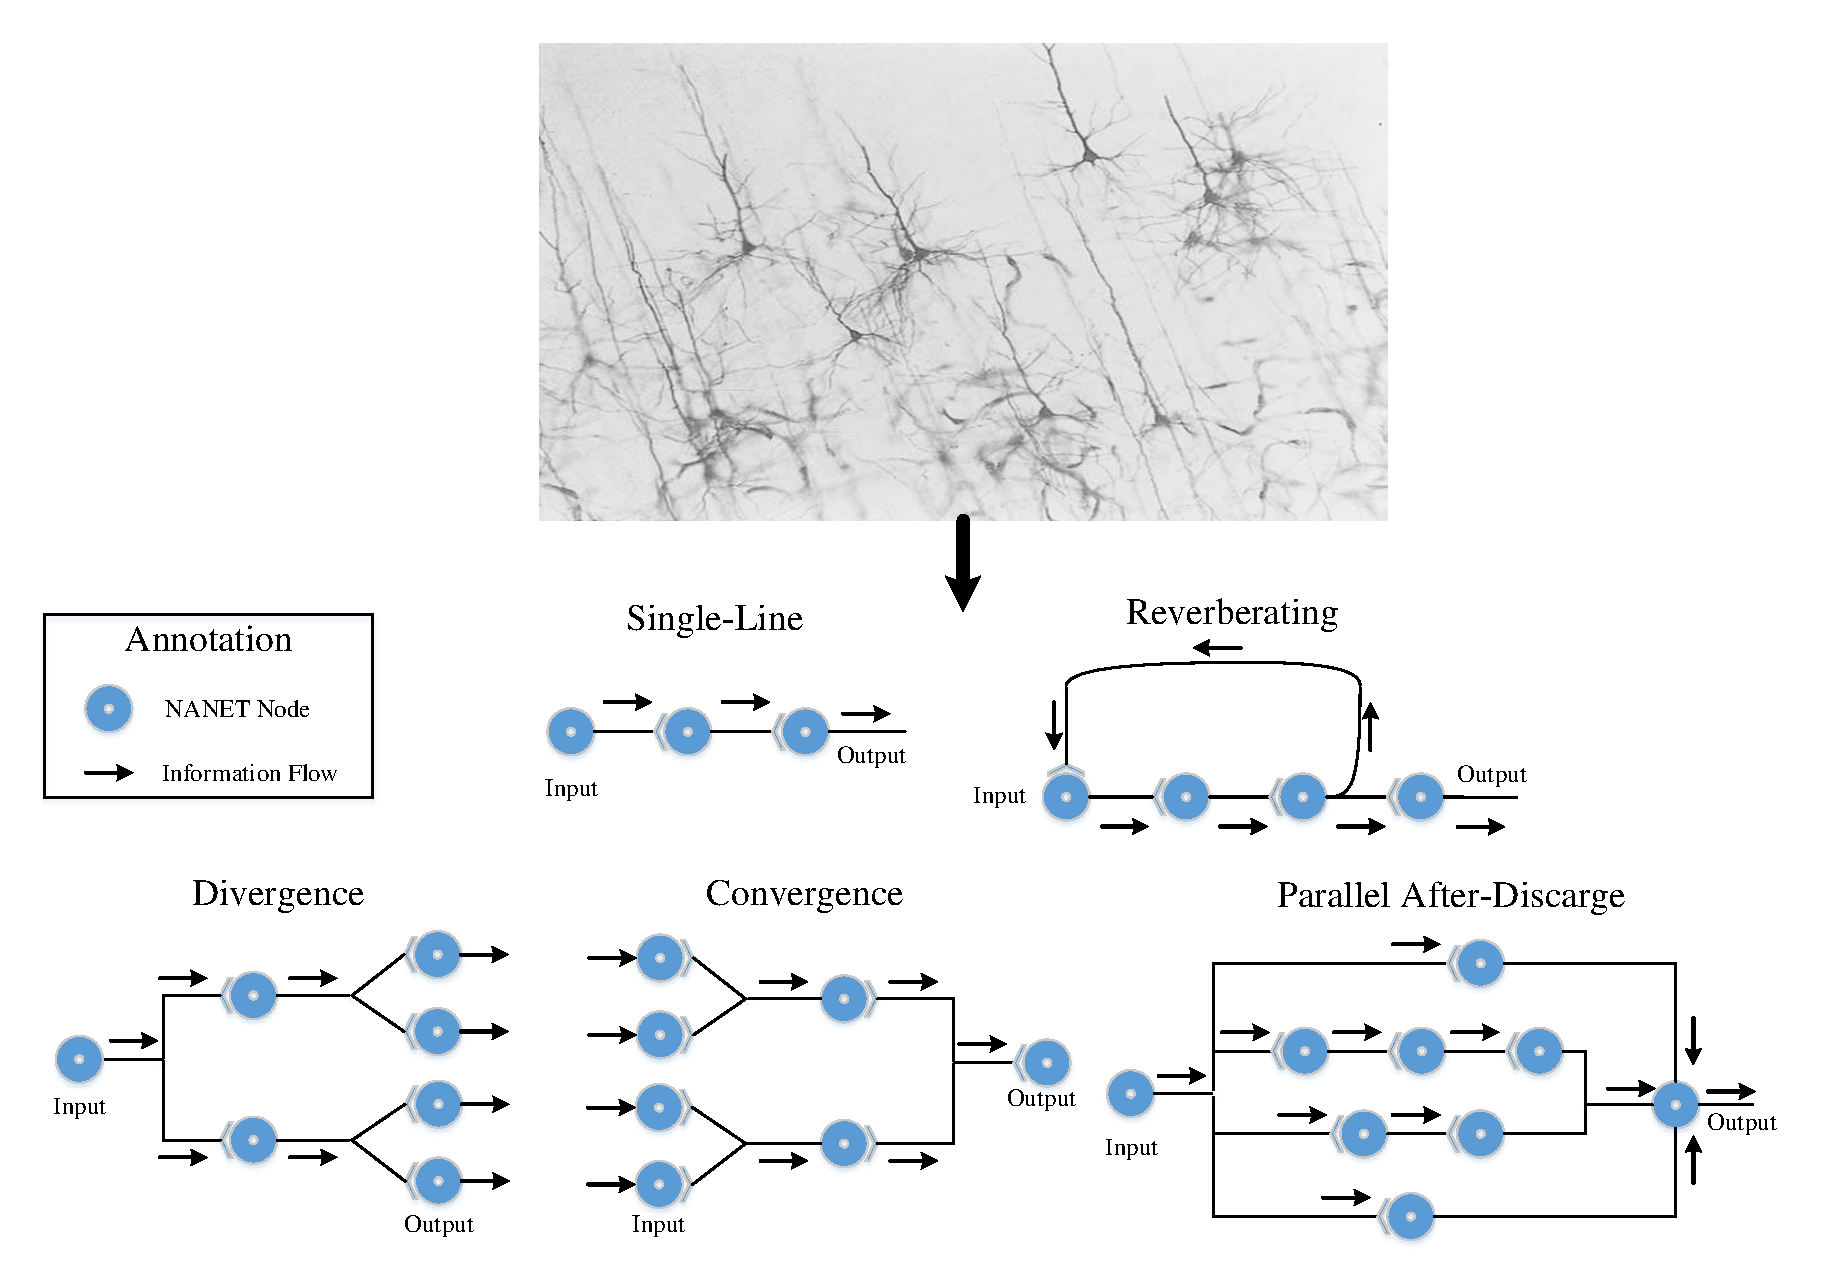
\includegraphics[width=\linewidth]{figures/tran_protocol.pdf}
				\caption{Transport Protocol Analogy of NANET and Neuron Network.}	
				\label{fig: transport_pro}
			\end{figure}
			As is shown in the Fig. \ref{fig: transport_pro}, transmission mechanism of neuron information mainly includes single-line transmission, convergent transmission, parallel transmission, and a small amount of divergent transmission.
			Among the diverse transmission mechanism, the single-line transmission is mainly the information transmission between two interconnected and independent neurons, while the divergent transmission is mainly the neurons distribute the information to the surrounding neurons in a broadcast-like pattern, using the surrounding neurons to assist in the information's forward dissemination.
			The neuron network receives a variety of inputs with time and space diversity, and  generates a particular output after a complicated and complex information fusion.
			Accordingly, the parallel transmission is a collaborative way through the participation of multiple sets of network nodes, which is similar to the core thoughts of network coding.
			In the single-line transmission,  it's analogous to the point-to-point transmission that is commonly used in communication, because the information only interacts between two nodes,
			Transmitting information through the participation of other nodes, the divergent transmission can be analogized to the distributed mimo at the physical layer, which can improve the system spectrum efficiency and transmission reliability, expand the scope of information dissemination.
	
	\section{The Integral Design and Goals of Neuron Analogy Mobile Ad Hoc Network}
	\label{section: general_design}
		In this section, we propose a kind of neuron analogy HWN(\ref{fig: sys_frame})  after the analogy of neuronal information transmission mechanism and HWN.
		For the entire NANET, we introduce certain goals and techniques in the level of network topology, user service, and transmitting contents.
		
		\subsection{Design of NANET Node}
				Fig. \ref{fig: NANET_node} shows the model of NANET node we proposed.
				\begin{figure*}[htbp]
					\centering
					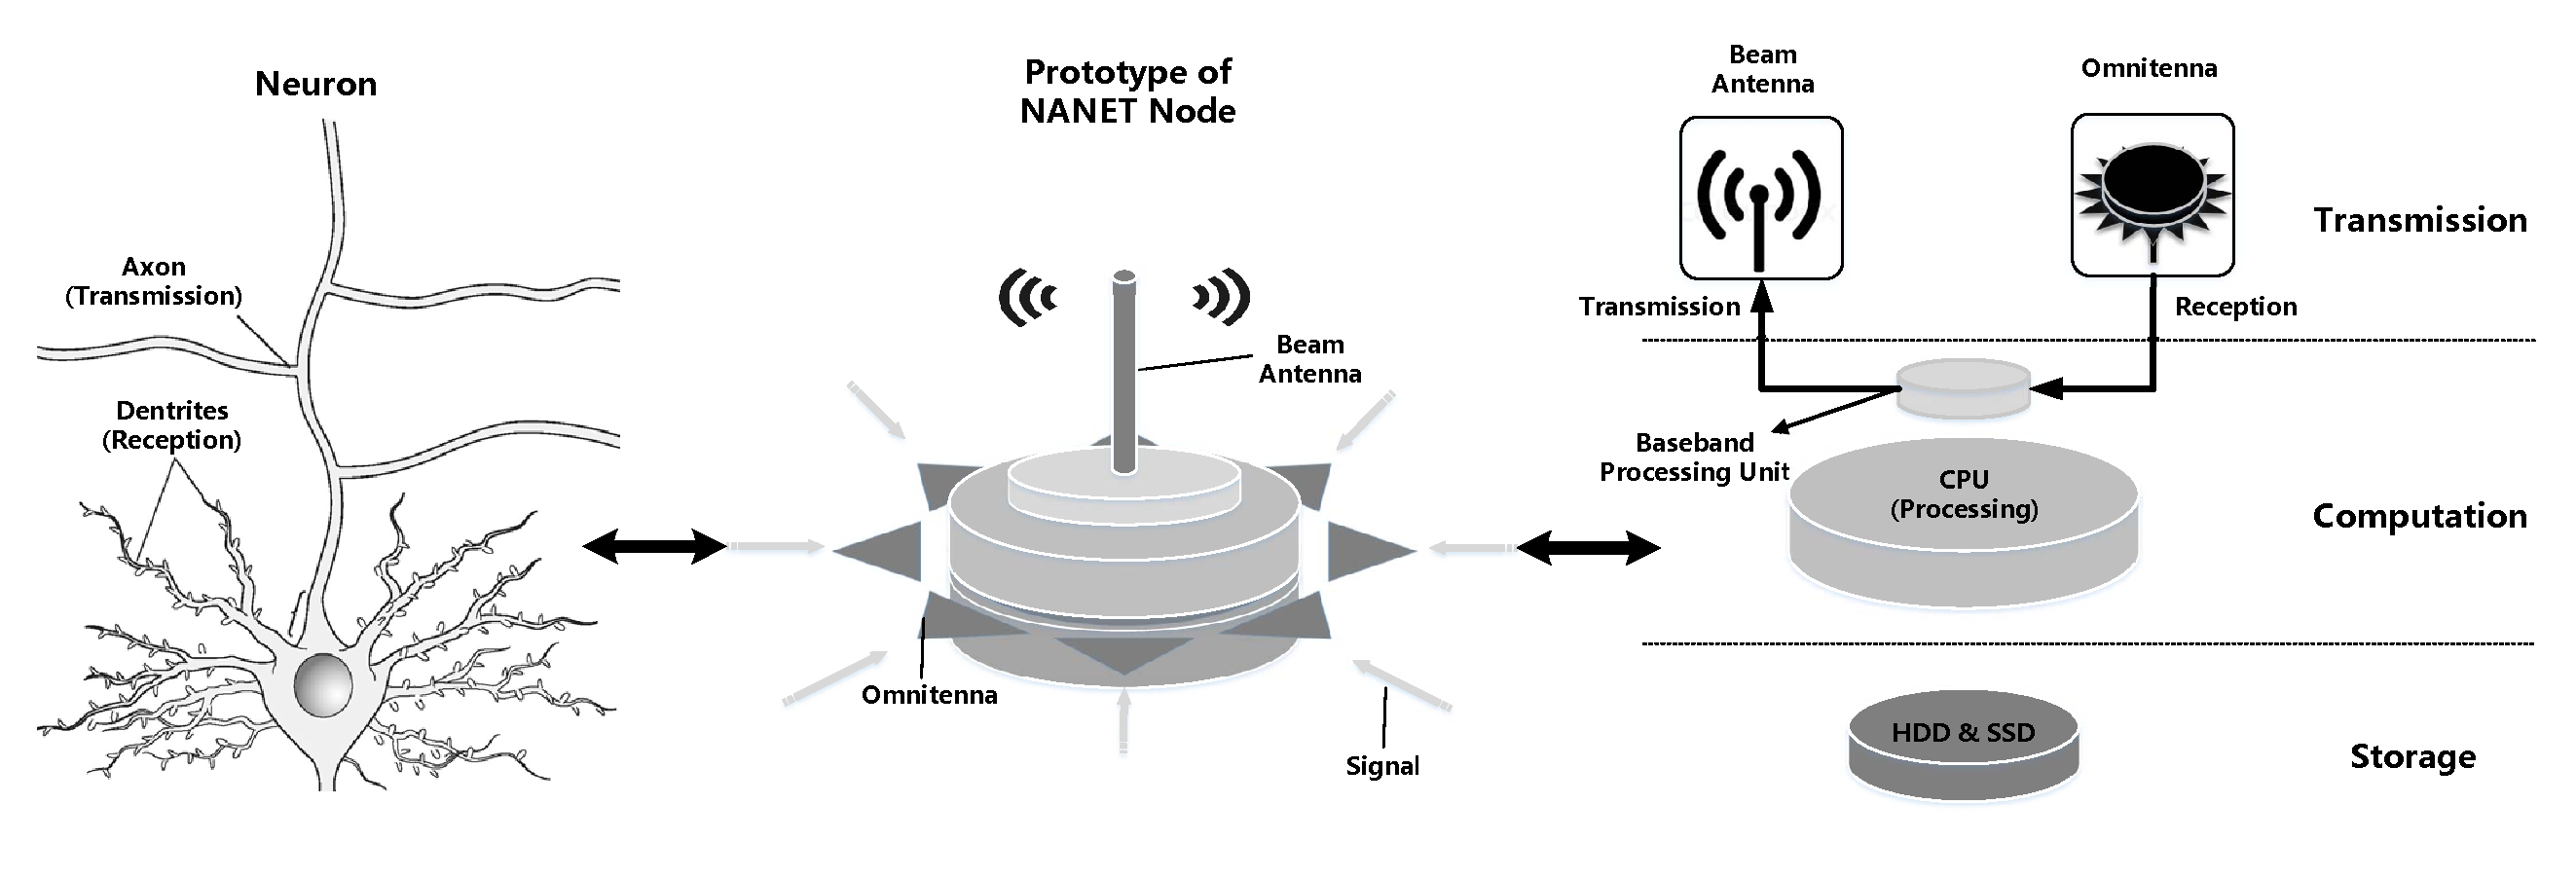
\includegraphics[width=0.95\linewidth]{figures/node_model.pdf}
					\caption{Design of NANET node.}	
					\label{fig: NANET_node}
				\end{figure*}
		
			\subsubsection{Design of NANET Node Structure}
				In the Fig. \ref{fig: NANET_node}, we can find out that there is a small vertical stick in the middle of the node. 
				It's the omnidirectional antenna of NANET node corresponding to the axon of the neuron node, and we can broadcast and forward information omnidirectionally.
				There are many a blocks pointing in all directions at the bottom of the NANET node, which denote directional antenna. 
				Corresponding to the dendrite of the neuron node, they can receive information form different directions.
				Following, it is the baseband processing unit(BPU) for the smallest y area connected with directional antennas in the center area of NANET node,
				which is mainly used for preprocessing of information reception and information processing, such as the signal amplification, etc.
				Below the BPU, the light gray cylinder represents the CPU that is utilized to process the signal to transmit or receive, for example, the fusion of signals from multiple directional antennas..
				At the bottom of NANET node, there exits a dark gray cylinder euqipped with the storage or cache capability of processing data or computing results.
				Certainly, the nodes would vary in the shape and function to feed the service requirements.
				For instance, the communication nodes would strenghthen their transmission ability emerging a higher communication capacity, while the computation node would build up the computing power.
				Accordingly, we would alter the shape of node to fit for the functional requirements of the network, and then node's heterogeneity appears.
				
			\subsubsection{Design of Information Transmission and Reception Mechanism in NANET Node}
				In the design of NANET nodes, the information transmission and reception are uncoupled guaranteed by the seperation of transmission antenna and reception antenna.
				As for the transmission antenna(in control backbone node? not clear), it's the omnidirectional antenna with larger power than the reception antenna, and transmit the information with in a broadcast form. 
				And it also assists other nodes in the transmitting information when forwarding its own received information, which can achieves the effect of cooperative transmission between the nodes.
				Information reception of NANET node utilize multiple directional antennas to separate different channels and receive information through specific orientation. 
				To some extent, multi-channel antennas' application could contribute to the reducing interference as well as facilitating the fusion of multi-channel information.
				And the multichannel reception would effectively promote the spectrum efficiency, transmitting speed, and QoS in NANET.
				Certainly, from the perspective of MIMO, it can exploit the spatial degrees of freedom provided by the multi-channel transmission channel.
				In certain, we also enhance the capabilities of storage and computation  in NANET node, so that it has the fusing and processing capabilities in application layer.
				Hence, in the NANET, information transmission is cooperative among nodes,  and broadcast and singlecast are combined with each other.
				
			\subsubsection{Design of Information Fushion and Processing}
				As shown in Fig. \ref{fig: NANET_node}, the received information of NANET node is based on the parallelled information fusion and processing in the processing unit.
				When the fusion of multi-channel information received by directional antenna satisfy certain conditions, for example, approaching the threshold, 
				the NANET node will foward or store the fused information, which is similiar to the production of the action potential.
				In order to reinforce the anti-interference ability, the information is encoded with the frequency of electromagnetic wave.
				In particularly, the information could be encoded and transmitted with several NANET node in cooperation with each other, as is done by network coding.
				Once the node decide to foward the infromation, the infrormation would be trasmitted in a constant power.
				The merged information is forwarded after the accumulated information reaches a certain threshold or the waiting time meets a certain triggering mechanism, 
				which is similar to the generation of action potential until the accumulation of incentive information approaching a threshold in our neurons.
				
				Therefore, the NANET node model we proposed, is an intelligent node equipped with transmitting, processing, and storage(Fig. \ref{fig: NANET_node}).
				The transmission and reception of information are separated.
	
		\subsection{Design of General NANET Architecture}
			
			In the following, we propose a NANET architechture with the trinity of space, air, and groud based on the analogy to the biological neural network.
			Fig. \ref{fig: sys_frame} shows the general design of NANET architecture from the macro perspective.
			\begin{figure*}[htbp]
				\centering
				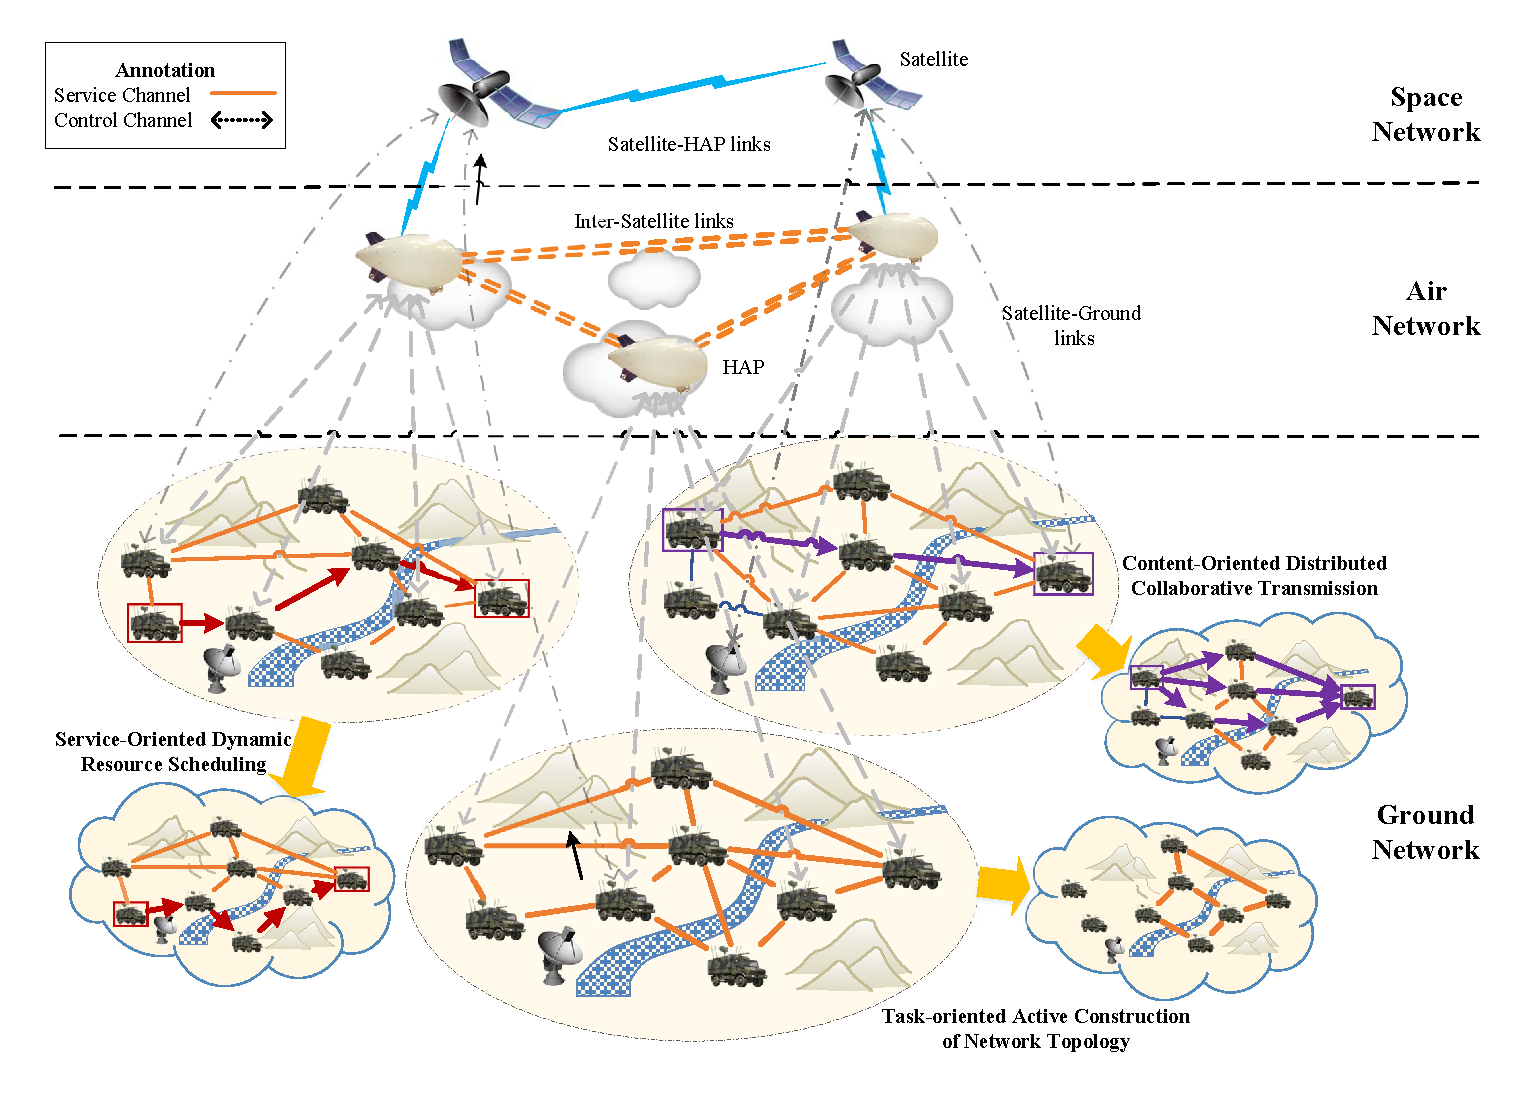
\includegraphics[width=\linewidth]{figures/Net_Arc.pdf}
				\caption{The design of general NANET architecture, which contains space layer, air layer, and groud layer, reveals the features of NANET structure and the design goals of NANET.}	
				\label{fig: sys_frame}
			\end{figure*}
			\subsubsection{Scale-Free Network}
				Any naturally growing network would tend to developing into a scale-free network, such as transportation network, highway network, etc. 
				It's primarily due to that the scale-free network is a good compromise for robustness and transmission efficiency.
				As a space-air-groud integrated network, NANET contains large-scale changing links among NANET nodes.
				Lengths of links differs from each other, and subjects to power distribution as well. 
				At the same time, density of nodes or links varies in different locations.
				Meanwhile, the bulk of the links possess a short average path length and the majority of nodes can cluster in a relatively small zone, which subjected to small-world property.
				
			\subsubsection{Seperation of Service and Control Channels}
				In the information transmission of NANET, the service channel is separated from the control channel.
				Generally, the control channel perform as a synchronization mechanism for information transmission of multiple nodes, 
				and information transmission in control channel is bi-directional, fast, and reliable when compared with service channel.                  
				Signaling information does not require further amplification due to its shortness.
				And it can't be processed, that is, it has the characteristic of unchangeability .
				Moreover, the property of reliability and unchangeability can be further guaranteed at the protocol level.
				On the one hand, wired channels can be used as control channel in ground for its highest transmission speed.
				On the other hand, the satelite or airship links can serve as control channel as wel,l while the links among genenral node play the part of service channels, 
				which realizes the characteristic that control channel is dramatically faster than the service channels.
				Because the ground node might require many hops to reach the target node for most nodes while the satellite node can almost connect to any node by one hop.
				Thus, the transmission efficiency of satellite communication is the highest, and its delay may also be affected by the number of hops which is much lower compared to the ground network.
				Of course, its resistance to damage and robustness are the worst, too.

			\subsubsection{Distributed and Centerless Network Framework}
				The NANET is a distributed network without a strict control center, all nodes of which have relatively equal status.
				And the property of distribution is reflected in the distribution of network framework and the distribution of information transmission.
				The NANET is a self-growing and self-organizing network, which determines that the network structure is unlikely to be a centralized network.
				Owing to fullfilling various requirements of service in different areas, the NANET would develop into a distributed network in network framework.
				Meanwhile, the information transmission in NANET is collaborative and distributed as well, which can greatly promote the efficiency of information transmission.
				However, non-center dosen't denote absolute equality or sameness for all of the NANET nodes.
				On the whole, the NANET always possess the backbone network from the perpective of entire system architecture.
				
			\subsubsection{Hierarchy and Heterogeneity of Network}
				Heterogeneity is not only a challenge but also an opportunity. 
				Homogeneous networks are difficult to adapt to the uncertain requirements of complex time-varying transmission, processing, and control.
				To address these problems, it is necessary to employ different networks which bring about the adaptability to situations the network meeting.	
				And then, only the heterogeneous network can satisfy various users' requirements of service or functions.
				Above all, hierachical networks are expedient to manage and plan to some extent.
				As shown in Fig. \ref{fig: sys_frame}, the NANET would be growing hierachically of its own accord, 
				as there are naturally three layers in the network: the space layer(satelites), the air layer(airships, airplanes, UAVs, etc.), and the grond layer(random access network).
				Hence, the NANETs can naturally form a hierarchical and heterogeneous network structure  according to the network scale.
				
			\subsubsection{Adaptability of Network Structure}
				
				From the perspective of network's adaptability, nodes can join and leave the NANETs scope at any time, 
				and the impact of the exit of any node or even partial of total nodes in the system could be negligible.
				With constantly changing of the network topology,  NANET is a resilient network with dynamically reconstructed resources.
				And in a sense, its resilience to damage and robustness are very strong.
				These variations come from the plasticity of NANET nodes, because the function and performance of node can be modified for short and long periods.
		
		Therefore, the information transmission of the space-air-land integrated NANET is equipped with the characteristic: separation of Service channels and control channels, combination of wide and narrow bands, integration of long and short links.
		It's a compromise between robustness and transmission efficiency.
		
		\subsection{Design of Transmission Protocol of NANET}
			\subsubsection{Transmission Synergy in Physical Layer}
				In summary, this information transmission in neuron network is based on the information fusion and cooperation of distributed neuron cells.
				
				The transmission mechanism of neuron information mainly includes single-line transmission, divergent transmission and a small amount of convergent transmission.
				Among the diverse transmission mechanism, the single-line transmission is mainly the information transmission between two interconnected and independent neurons, while the divergent transmission is mainly the neurons distribute the information to the surrounding neurons in a broadcast-like pattern, using the surrounding neurons to assist in the information's forward dissemination.
				
					When omnidirectional, let the people on the edge have the opportunity to participate in the decision-making process as much as possible, and receive the channels to isolate them in order to facilitate the fusion process.
				This not only facilitates distributed and cooperative transmission and fusion processing, but also helps suppress the mechanism of multi-channel interference.
				Embodies the simplicity of transmission.
			\subsubsection{Coding Synergy in Network Layer}
				Neuronal cells receive thousands of synaptic inputs that activate different combinations of receptor proteins and their corresponding ion-gated channels on the cell surface.
				It namely means that neuronal information transmission is related to combination of activated channels and receptor proteins, which is similar to the network coding in our information network. 
				Through the information transmission between multiple network nodes, it is allowed to encode and fuse the information from different links. 
				Thus, the combination of all link information constitutes the complete information.
				Network coding enables HWN nodes to achieve both coding and routing functions,In terms of the concrete transmission mechanism, the NANET would imitate the physical transmission mechanism of neurons 
				to achieve integration of different regional networks and distributed cooperative transmission of information.
				
				For content-distribution applications in the network, its content obey the twenty-eight flow distribution law.
				The current network mechanism is in a end-to-end transmission manner. 
				In the transmission process, the network is not memorized, and its content is not perceived which will lead to a large amount of repeated transmission of content.
				Network traffic will exponentially increase eventually if not changing the transmission mechanism. 
				And we cannot solve the exponential growth of traffic because of the linear expansion of the network capacity.
				
				The HWN network is a integrated network of time, space, and frequency.
				Spectrum resources are limited. This requires us to make reasonable use of spectrum resources.
				Through multiple levels of multiplexing of spectrum resources, such as time, space, and frequency, the utilization efficiency of communication resources is improved, and time-space-frequency integrated information transmission is realized.
				So it's necessary for us to make reasonable use of spectrum resources, and to increase the utilization efficiency of communication resources through the multiplexing of spectrum, such as the integration of time domain, space domain, and frequency domain, as the neurons does in dendrites' information integration.
				
				The HWN network is an integrated network of sky, air, and ground. 
				The integration of sky, air, and ground not only enables the network to have large-scale changes in scale,
				but also enlarge the coverage range of the network.
				And it could conduce to the combination of the control channel and the Service channel, which would in turn contribute to the cooperative transmission of the content.
				
				The HWN network is a network with links, networks and service integrating.
				Through the computation and storage capabilities of network nodes, HWN networks can perceive and comprehend the contents that application distributes and user requests.
				It's essentially a cross-layer collaboration of the network layer and the application layer, 
				which will be conductive to alleviate or solve the exponential growth problem of traffic and bring about a series of  institutional optimizations of traditional content distribution.
				
				Therefore, the NANET is a content-oriented network with a distributed cooperative transmission mechanism. increase the network throughput, 
				contribute to load balancing, and improve network bandwidth utilization.
				
			\subsubsection{Content Synergy in Application Layer}
				The HWT is a network where their nodes integrate ability of transmitting, storage, and computation.
				In some cases, computation resources and storage resources can be exchanged for bandwidth resources, such as what have been done in content distribution network (CDN). 
				With the ability of fusing and processing for HWN node, we can use the node's capability of storage to cache user-requested content in the network nodes where users relatively concentrated in, and respond to users' real-time requests. Thus, users can be adequate to obtain the content requested in the surrounding nodes, which would improve the efficiency of the user's acquisition of data resource.
				And then, HWN would naturally come into being a content distribution network, promoting the intelligent flow of content in NANET.
				In the application layer, the content distribution based HWN, would redirect the user's request to the service node closest to the user himself/herself, according to the network traffic, links status, load distribution, response time, etc.
				In this way, the user can get the desired content nearby, which at the same time can alleviate or solve the issue of network congestion, improve the response speed of the user's requests for services and resources, and greatly improve the efficiency of resource utilization.
				Therefore, information distribution of NANET can realize distributed fusion processing and cooperative transmission.
		
		\subsection{Design Goals and Techniques for NANET}
		\label{section: framework}	
		%	From the perspective of network topology, we hope that the AN-HWN network can construct the network topology actively for specific tasks and achieve the appropriate network transition.
		%	For specific services, resources can be dynamically allocated to achieve on-demand resource allocation;
		%	Content-oriented, distributed and collaboratively transmitted, to ensure the quality of service of users.
			
			\subsubsection{Task-oriented Active Construction of Network Topology}
			
				%				The basis of communication networks is routing. 
				%				Generally, routing is usually used for sensing the network topology and perceiving the network state.
				In terms of network topology, the topology of NANET we proposed is oriented toward specific tasks.
				The overall idea is to build a control channel that is independent of the traffic channel as the control backbone network of the network topology.
				After each node in NANET obtains its own status, it reports the status information to the control backbone network with the control channel.
				The information of each node is gathered at the control backbone network, and the topology of the network is dynamically planned and adjusted in a quasi-real-time manner according to the system requirements.
				Then, the control node delivers the signaling of topology information to relevant nodes within the NANET.
				Following, corresponding nodes would regulate their own state according to the control signaling to realize the macro network topology adjustments.
				In this way, we can actively recognize and control the topology of NANET in real time,.
				There exits many advantages for NANET.
				On the one hand, the system overhead caused by the cooperation of multiple groups of Service channels through the control channel is much smaller if compared with the cost of routing, 
				and the network topology can be perceived and controlled in real time.
				On the other hand, since the current network topology is actively constructed by the NANET itself, the topology is required for the current task specially, 
				which means a greatly improvement on the efficiency of information transmission and a quick achievement of current task. 
				The tasks that the network needs to perform.
				
				In summary, the NANET we proposed would possess a strong adaptability with perceiving the real-time network state and actively constructing the network topology.
				We can make use of complex networks, dynamics, and other theoretical tools to equip the network with the ability to actively constructing the topology, 
				and compromise the conflict between heterogeneity and complexity of the network.
		
			\subsubsection{Service-Oriented Dynamic Resource Scheduling}
			
				In terms of resource scheduling, we envisage that NANET would establish a dynamic pricing mechanism gradually,
				which can be used to convert network resources into corresponding value and supply users corresponding value of network resources according to the user's payment.
				It's similar to present traffic network on the flow planning when the HWN is specialized to each point-to-point transmission of Service information.
				Maybe, in one place, the roads are wide, but they often undergo traffic jam.
				While in another place, the roads are narrow, but their traffic system is very efficient.
				Therefore, when the flow reaches a certain level, the width of the road is not a decisive factor in determining the efficiency of traffic.
				For wireless networks, each node in the network is selfish, and this selfishness drives the node to achieve the information transmission employing communication resources with the least self-loss.
				The node's pursuit of minimal loss itself causes the competition among different nodes 	due to the limitation of total amount of resources.
				From the perspective of the entire network, the competition is unbalanced for degree of competition in different local areas of the network varies greatly. 
				It causes the network to be idle in some areas, while the network are blocked in the other areas.
				Therefore, we should introduce an approach of market economy, and borrow its mechanism of dynamic pricing to lead the allocation of network resource.
				Ultimately, we can use network resources more rationally to achieve a compromise between efficiency and fairness, and achieve a balanced flow across the world.
				
				Dynamic pricing is relatively easy to implement, but what's more difficult is to found a dynamic charging mechanism.
				Blockchain is a value-passing network, and had been proposed by Satoshi Nakamoto in 2008. 
				It is an intelligent peer-to-peer network that uses a distributed database to identify, disseminate, and document information. 
				Hence, we could use the relevant technology of blockchain to value network resources in NANET, and value the network resources to establish a natural competition mechanism.
				In the NANET, users can purchase the virtual currency, and they can obtain virtual currency through previous behavior on network resource utilization as well.
				For example, if a user decreases the network load, or facilitates load balancing, or improves resource utilization of whole network through his own actions, 
				NANET system would award the user a corresponding count of virtual currency as a reward to the user for his promoting overall performance of the network. 
				As for the mechanism of dynamic pricing and dynamic charging of resources, 
				we would naturally utilize the principles of economics to solve, such as the basic economics of Nash equilibrium theory in game theory.
				
				In short, in order to promote the utilization efficiency of network resources, 
				we would exploit some mathematical methods, such as game theory, to value network resources and charge users the virtual currency dynamically, according to the real-time status of the NANET.
				At last, NANET would realize a mechanism of scheduling network resources dynamically.
				
			\subsubsection{Content-Oriented Distributed Collaborative Transmission}
			
				In terms of the concrete transmission mechanism, the NANET would imitate the physical transmission mechanism of neurons 
				to achieve integration of different regional networks and distributed cooperative transmission of information.
				
				For content-distribution applications in the network, its content obey the twenty-eight flow distribution law.
				The current network mechanism is in a end-to-end transmission manner. 
				In the transmission process, the network is not memorized, and its content is not perceived which will lead to a large amount of repeated transmission of content.
				Network traffic will exponentially increase eventually if not changing the transmission mechanism. 
				And we cannot solve the exponential growth of traffic because of the linear expansion of the network capacity.
				
				The NANET is a network where their nodes integrate ability of transmitting, storage, and computation.
				In some cases, computation resources and storage resources can be exchanged for bandwidth resources, such as what have been done in content distribution network (CDN). 
				The capabilities of node's storage and computation make users adequate to obtain the content requested in the surrounding nodes, improving the efficiency of the user's acquisition of data resource.
				Consequently, we would equip the node of NANET with the ability of transmitting, storage, and computation, which is similar to  what we have been doing in so-called 3C integration.
				Thus, the node would have the memory function and be adequate to store content, which can promote the intelligent flow of content in NANET.
				
				The HWN network is a integrated network of time, space, and frequency.
				Spectrum resources are limited. This requires us to make reasonable use of spectrum resources.
				Through multiple levels of multiplexing of spectrum resources, such as time, space, and frequency, the utilization efficiency of communication resources is improved, and time-space-frequency integrated information transmission is realized.
				So it's necessary for us to make reasonable use of spectrum resources, and to increase the utilization efficiency of communication resources through the multiplexing of spectrum, such as the integration of time domain, space domain, and frequency domain, as the neurons does in dendrites' information integration.
				
				The HWN network is an integrated network of sky, air, and ground. 
				The integration of sky, air, and ground not only enables the network to have large-scale changes in scale,
				but also enlarge the coverage range of the network.
				And it could conduce to the combination of the control channel and the Service channel, which would in turn contribute to the cooperative transmission of the content.
				
				The HWN network is a network with links, networks and Service integrating.
				Through the computation and storage capabilities of network nodes, HWN networks can perceive and comprehend the contents that application distributes and user requests.
				It's essentially a cross-layer collaboration of the network layer and the application layer, 
				which will be conductive to alleviate or solve the exponential growth problem of traffic and bring about a series of  institutional optimizations of traditional content distribution.
				
				Therefore, the NANET is a content-oriented network with a distributed cooperative transmission mechanism.
			
	\section{Conclusions and Visions Future}
	\label{section: Conclusion}
		Recently, mobile ad hoc network is attracting lots of research attention in multiple fields with the development of internet of vehicles as well as internet of things. 
		However, the performance of HWN would decrease exponentially with the increasing of nodes' number and mobility due to the time-varying of network topology and uncertainty of service requirement. 
		In this paper, we firstly introduce the information transmission mechanism of neural netwroks, 
		and compare the mechanisim with that of mobile ad hoc network, 
		including the node model, network structure, and transmission protocol. 
		And then, we propose the Neuron Analogy Mobile Ad Hoc Network(NANET) and provide its overall design of node and network architecture simultaneously.
		In addition, we depict the overall design goals and related feasible technologies.
	
	
	\appendices
	\section*{Acknowledgment}
	This work is financially supported by Natural Sciences and Engineering Research Council of Canada (NSERC) and National Natural Science Foundation of China (91638204).
	
	\nocite{*}
	%	\bibliographystyle{IEEEtran}
	%	\bibliography{5G_spectrum_sharing}
	
	
	% Can use something like this to put references on a page
	% by themselves when using endfloat and the captionsoff option.
	\ifCLASSOPTIONcaptionsoff
	\newpage
	\fi
	\bibliographystyle{plain}
	\bibliography{bib/tex}
\end{document}